\documentclass{article}
\usepackage[left=2cm, right=2cm, top=2cm]{geometry}
\usepackage{amsmath}
\usepackage{amsfonts}
\usepackage{graphicx}
\usepackage{color}
\title{Response to Reviewers: Manuscript ID 17-1142.1: ``Learning Augmented Joint-Space Task-Oriented Dynamical Systems: A Linear Parameter Varying and Synergetic Control Approach"}

%\author{Your Name  \\
%	Your Company / University  \\
%	\and 
%	The Other Dude \\
%	His Company / University \\
%	}
%
%\date{\today}
% Hint: \title{what ever}, \author{who care} and \date{when ever} could stand 
% before or after the \begin{document} command 
% BUT the \maketitle command MUST come AFTER the \begin{document} command! 
\begin{document}
\maketitle
First of all, we would like to thank all reviewers for the time they spent reviewing our paper. We greatly appreciate the comments, suggestions and opinions that we received. We have addressed all the necessary comments and suggestions in the attached manuscript accordingly.\\
% % % % % % % % % % % % % % % % % % % % % % % % % % % % % % % % % % % % % % % % % % % % % % % % % % % % % % % % % % % % % % % % % % % % % % % % % % % % % % % % % % % % % % % % % % % % % % 
\noindent \underline{Comments from Reviewer \#1 (Reviewer: 4 (Review30069)):}
\begin{enumerate}
\item \textcolor{blue}{\textit{``As mentioned by the authors, there are many reasons to plan in joint space rather than task space. One of the important reasons to me seems to be able to plan end-effector orientation, not just position. Traditional movement primitives, for example DMPs, do not explicitly encode planning in the SO(3) space of orientations. There is research that addresses this question, for example [1], but they lose the simplistic appeal of movement primitives. I think it would be a great addition to this paper if the authors illustrate if their joint space DS can be used to accomplish orientation sensitive tasks, and generalize to end-effector orientations different that what was demonstrated.[1] Ude, Ale, et al. "Orientation in cartesian space dynamic movement primitives." Robotics and Automation (ICRA), 2014 IEEE International Conference on.}}"\\
\texttt{Response:}  We highly appreciate this comment. When we initially proposed this approach, we did not think about tackling the problem of reaching a target in orientation as well. Since our DS is learned in joint-space, indeed, we do not have to deal with the challenges that arise when trying to reach a target in both position and orientation as we do not have the constrains imposed by SO(3). There was theoretically no modification needed in our controller:
\begin{equation}
\underbrace{\dot{q}}_{\mathbb{R}^{m\times 1}} = -\underbrace{\mathcal{A}(q)}_{\mathbb{R}^{m\times m}}\underbrace{J^{T}(q)}_{\mathbb{R}^{m\times d}}\underbrace{(H(q)-x^*)}_{\mathbb{R}^{d\times 1}}
\label{eq:jtds}
\end{equation}
Originally, when working solely in position $d=3$, now we represent the target with $d=9$, where the first 3 dimensions correspond to Cartesian position and the remaining 6 correspond to the first and second columns of a rotation matrix $R \in SO(3)$. This only modifies the Jacobian $J(q)$ which is now $J(q)\in \mathbb{R}^{9 \times 7}$ rather than $J(q)\in \mathbb{R}^{3 \times 7}$. The role of the $\mathcal{A}(q)$ and their meaning is the same.



\item \textcolor{blue}{\textit{``In the introduction, the authors stress that jacobian psuedo inverse
can be computationally expensive. Is this really true for a 7-dof robot
arm? Can the authors provide some numbers where this would really be an
issue for a robot controlled at 1000Hz? I find the argument that
jacobian inverse does not work for singularities and needs a set of
heuristics to be more compelling. Maybe the authors should rewrite the
introduction to stress more on this issue?"}}\\
\texttt{Response:} \small For a 7-DOF robot it is indeed negligible. Computational burden only becomes a real issue for higher degrees of freedom, like a multi-fingered hand or multi-arm robotic setting. We will remove this passage from the text as we don't have much space to discuss it....\\

\item \textcolor{blue}{\textit{``In Section II, criterion I, the authors talk about a positive symmetric matrix P. I do not see it in the
equations above. Is this a weighing matrix?"}}\\
\texttt{Response:} \small Removed, that was a carry-over from a previous formulation.\\

\item \textcolor{blue}{\textit{``In criterion II, the error is defined with respect to the velocity error, rather than a position or a combination
of both. This means that the motion can be different from the demonstrated motion. I understand
that this is important to keep the later optimization convex, but is there any disadvantage to using
velocity error rather than position error?"}}\\
\texttt{Response:} \small Optimizing for position distance alone would have the effect of learning a motion that converged to the average of previous motions, thus not changing the motion in new situations or fitting the joint velocity profile that is often a desired component of the motion. Using velocity error does mean that, for motions strongly dependent on joint position rather than joint velocity, the generated motions may generalize from the demonstrations in unexpected ways. However, as you mentioned, minimizing position error would, depending on the formulation, be prohibitively difficult. This would imply simulating the learned motion forward in time to recompute the robot's positions, making the optimization much more complicated; this way, we can treat each point in the motion independently.\\

\item \textcolor{blue}{\textit{`I do not completely understand the significance of A(q). From Figure 3, it seems like A(q) helps resolve
redundancy, while achieving the task space goal. Do the authors have a mathematical (in constrast to
intuitive) explanation for this? Does A(q) somehow relate to the null-space of the jacobian?"}}\\
\texttt{Response:} \small A(q) transforms a joint velocity vector approximately aligned with the task-space error into a different joint velocity vector that remains approximately aligned with the error, but which we want to choose to more-closely approximate our demonstrations. In this sense, it is resolving redundancy between all the possible joint velocity vectors that would move the controller closer to the origin. The paragraph in Section III has been modified to improve clarity. A(q) doesn't relate to the null-space of the Jacobian in any clear way, as its value can and does alter the task-space trajectory as well as the joint space trajectory. The only property that A(q) preserves is the joint velocity's moving the task space position closer to the goal, but the direction of motion is not necessarily the same as the direction of task-space error.\\

\item \textcolor{blue}{\textit{``In Section III, ?One can intuitively understand the control law as follows:$(H(q) - x^*)$ denotes the
position error w.r.t. the task target and by multiplying that error by the transposed Jacobian JT (q),
the error is projected into joint space (similar to Jacobian transpose control)?. I find this explanation
misleading as jacobian multiplied to position error does not project the error into joint space. Jacobian
transforms velocities, not positions. Maybe the law can be seen more as a first order approximation
of the error in task space. In any case, I would either clarify this statement more or take it out of the
manuscript all together. It seems like the DS is just a PD law that provably converges to a fixed attractor
in task space."}}\\
\texttt{Response:} \small The passage has been rewritten to remove the word "project", which you appropriately noted was incorrect, and further clarifies the nature of the DS as a PD controller. We have added the following text in the manuscript: 
\textit{``One can intuitively understand the control law as follows: $(H(q) - x^*)$ denotes the position error w.r.t. the task target, which we then reinterpret as the task-space velocity of a proportional controller. By multiplying that error by the transposed Jacobian $J^T(q)$, it is transformed into a joint-space velocity vector correlated with the error (similar to Jacobian transpose control [?]), see Fig. [?]. The positive definite matrix $\mathcal{A}(q)$ warps the resulting joint-space velocity; Fig. [?] illustrates the effects of  $\mathcal{A}(q)$ on the generated motion. Thus the controller can be thought of as a proportional controller in joint space.}\\

\item \textcolor{blue}{\textit{``About figure 2 again, the position error in task and joint space are not simply multiplied by a Jacobian.
Although, task space error can be first-order approximated using a Jacobian multiplication with
joint space error. What does the right figure in Fig 2 exactly represent?"}}\\
\texttt{Response:} \small The figure on the left is simply the cartesian error in task space. The figure on the left is the Lyapunov potential function on which the jacobian transpose controller descends. In showing the attractive regions in joint-space corresponding to this Lyapunov function, we aim to offer insight into how the controller reformulates the task-space potential into a different yet related joint-space potential. The caption has been rewritten to add clarity.\\

\item \textcolor{blue}{\textit{``In Section IV, the authors say that they use EM to determine the parameters of the GMM in Eq 6. Can
they elaborate a little on this? What is the expectation taken over and what likelihood is maximized?"}}\\
\texttt{Response:} \small The algorithm computes the expected probability of generating each of the joint positions given the current values of the GMM's means, variance matrices, and scaling values. The algorithm then chooses GMM parameters to maximize the posterior likelihood of the model, using previously-computed expected component membership as likelihood weights when computing the new mixture. Specifically, we used MATLAB's \textit{fitgmdist} implementation. Added a citation to clarify.\\

\item \textcolor{blue}{\textit{``The learned dimensionality reduction and parameters seem task dependant. I wonder if the authors
have any idea on how to generalize this across tasks."}}\\
\texttt{Response:} \small The dimensionality reduction could be generalized across tasks that had the same motor synergies - that is, for example, all tasks in which the shoulder and elbow always move together. Similarly, one could imagine several similar motions that could be decomposed into shared submotions, thus allowing the parameters to be shared. However, in general, fixing some of the parameters while optimizing will simply lead to a less-flexible model, and considering that there is no intuitive scheme for a-priori identifying motions with strongly similar submotions, we did not explore this question further. To answer your question directly, if one wanted to, one could reuse the learned dimensionality reduction for a new task which you believed to be similar, or copy certain components of a previous motion's GMM into the new GMM and leave them fixed throughout the optimization.\\

\item \textcolor{red}{\textit{``The experiments have the same task-space goal as the
demonstrations. Can the authors include experiments that have goals
different from demonstrated, especially in orientation?"}}\\
\texttt{Response:} \small First of all, they don't.. show some figures... add clarification of this in the text and explain why we cannot systematically evaluate this if we had too..\\

\item \textcolor{red}{\textit{``In similar light, maybe authors could present online adaptation of
A(q) to generalize to situations different than demonstrated, for
example a slightly moved obstacle?"}}\\
\texttt{Response:} \small This is a really nice suggestion. But how I see it, it's basically a new paper; i.e. an extension of this one, but we can discuss about this if we have space. A quick idea that comes to mind would be to apply a modulation/activation to the LPV system in a local region. Now this is not as straight forward as in our task space approaches because our LPV system is learned in joint-space while the activation function is in the embedded space. Another idea is to modify the activation function of the local behavior regions such that it is a function of an external variable, for example if force is applied/sensed, and it bias the model towards another $A_k$ matrix? So it still would be an open question, but an approach to tackle this problem could be along these lines.... Add a passage in the discussion answering this question\\

\item \textcolor{red}{\textit{``In table II, instead of the tracking error, maybe the more useful
error to see would be the error with respect to the plan or
demonstartion. One would assume that the proposed approach would be
worse at it than SEDS+IK because the minimized error is with respect to
the velocity and goal, not the position of the movement."}}\\
\texttt{Response:} \small This is not necessarily the reason that it would be worse, as SEDS is also learned by minimizing the error with respect to
the velocity and the goal. The reason that JT-DS is less accurate in reproducing the motion in task-space is because our optimization is focused on reproducing the motion solely in joint-space, while reaching the final target in task-space. Nowhere do we claim that JT-DS is capable of reproducing a motion in both joint and task space. Nevertheless, we add the mean swept-error-arrea (SEA) which evaluate the performance of reproduction in task-space from a reference trajectory... as shown in the tables....\\
\end{enumerate}

% % % % % % % % % % % % % % % % % % % % % % % % % % % % % % % % % % % % % % % % % % % % % % % % % % % % % % % % % % % % % % % % % % % % % % % % % % % % % % % % % % % % % % % % % % % % % % 
\underline{Comments from Reviewer \#2 (Reviewer: 5 (Review30371)):}
\begin{enumerate}
\item \textcolor{blue}{\textit{``My first concern regards you choice of representing the demonstrated
movement as a sequence of postures and hence looking for synergies by
using PCA of K-PCA analysis. Why not using functional PCA (f-PCA)
analysis and determine the few moving synergies that make possible the
execution of the demonstrated behaviours? It would be that, when you
combine the local synergies in space and time by using functions
$\theta_k(q)$, you get what you might obtain by using directly f-PCA.
However, the last one are valid for the whole movement and can be
combined by constant coefficients."}}\\
\texttt{Response:}  See below.

\item \textcolor{blue}{\textit{``I also found the paper lacking of physical intuitions, especially in	the experimental part, about the entities introduced in previous sections. In particular, what is the lesson we learn after your analysis of synergies and the obtained lower dimensional space for the few movements shown in section V? Is it possible to extract some global	synergic behavior? Moreover, in section IV.A authors introduce the function phi(q) named the embedding that maps the joint configuration into a lower dimensional space. Is it associated to a whole behaviour or, as matrices $A_k$, has a local validity? I lost this point. Can you show/report or describe what it represents in the joint space for one or more cases in Section V? What is this lower dimensional space for the cases in Section V?"}}\\
\texttt{Response:}  See below.		

\item \textcolor{blue}{\textit{``A similar question for the matrices $A_k$ that represent local, I
	would say postural (see previous comment), synergies whose dimension is
	m x m, i.e. in joint space: I would expect they were defined in the
	lower dimensional space. Moreover, are they local representation of the
	distribution of postures and hence covariance matrices? What do their
	eigenvectors and eigenvalues locally represent? Maybe, a comparison
	with the classical and more known postural synergies for the human
	hand, analyzed by PCA, could be useful. Finally, what does it mean that
	they should be positive definite (apart from stability issue)?"}}\\
\texttt{Response:}  See below.\\

\item \textcolor{blue}{\textit{``What is the dimension of function $\theta_k(q)$ that, to some extent, can be seen as the new control variables. Is it $K<m$?"}}\\

\texttt{Response:} In response to Comments 1-4, following we mathematically and graphically analyze the proposed local behavior synergy extraction scheme which is composed of dimensionality reduction of the joint trajectories (via. PCA or K-PCA) and grouping of local behavior regions with GMM on this lower dimensional space. The $K$ clusters found in this embedded space correspond to the number of $K$ synergy matrices that will parametrize $\mathcal{A}(q)$. Let's begin by analyzing the proposed DS-based control-law \eqref{eq:jtds}. The intuition behind this control-law is that $\mathcal{A}(q) = \sum\limits_{k=1}^{K}\theta_k(\phi(q))A_k$ is a linear combination of time-invariant linear matrices $A_k \in \mathbb{R}^{m \times m}$, \underline{these matrices are the ``local behavior synergy matrices"} that shape the motion in joint-space. Meaning that, given the joint-space velocity vector representing the task-space error $J^{T}(q)(H(q)-x^*)$, the resulting motion is biased to use a particular set of joints, defined in each $A_k$. Each $A_k$ is thus activated depending on the current ``joint-posture" $q$ (represented in the lower-dimensional space $\phi(q)$) via the scheduling/activation function $\theta_k(\phi(q))$.
$\phi(q)$ is a learned transformation, which is associated with a whole behavior, rather than a particular $A_k$ (as is now clarified in IV.A). However, the precise nature of the transformation depends on the DR technique: PCA applies a uniform matrix multiplication of joint position everywhere, whereas KPCA is a more complicated function of joint position.  The result of the embedding is a lower-dimensional representation of the joint position. The following line has been added to IV.A for clarity:
\textcolor{blue}{\small \textit{"For example, if the shoulder and arm joints are coupled throughout the motion, and $\phi(\cdot)$ were a matrix multiplication, it could map the "shoulder" and "arm" components of $q$ into a single "shoulder-arm" component in $\phi(q)$.}"}

Given the raw demonstrations of a joint-space  behavior with a task-space target as shown in Fig. \ref{fig:raw_demos} (for the pouring task) we seek to learn a linear combination of local behavior synergies $\mathcal{A}(q) = \sum\limits_{k=1}^{K}\theta_k(\phi(q))A_k$ such that we can use \eqref{eq:jtds} to accurately reproduce these demonstrations. In order to do so, we project the raw joint trajectories to a lower-dimensional space via $\phi(q)$, in the case of PCA $\phi(q)=M_p \times q$ for $M_p \in \mathbb{R}^{p \times m}$. By choosing the first 3 PCs we can explain 95\% of the variance in the joint posture trajectories, which can be represented in this 3-D space as shown in Fig. \ref{fig:raw_demos}. We then jointly learn the activation function $\theta_k(\cdot)$ and the number of $K$ local synergy regions by fitting a GMM to this representation of the joint posture trajectories. As can be seen in Fig. \ref{fig:raw_demos}, the entire joint-space motion can be represented by 3 local synergy regions in PCA-space. Meaning that we only need 3 synergy matrices $A_k$ to represent the complex joint-space motion accurately. The activation function $\theta_k(\cdot)$, as described in the mansucript, is the posterior probability of a joint posture in PCA-space $\phi(q)$ belonging to one of the local synergy regions $k \in \{1,\dots,K\}$. As mentioned in Sec. V.A., we treat K as a hyperparameter and thus choose it differently for each learned motion. For motions that do not vary much throughout the course of the motion, smaller K might be sufficient, but K can just as easily be greater than $m$ (though as $K$ increases, so does the learning problem's computational cost). If comment-4 was about each specific $\theta_k(q)$, they are scalars, as is mentioned in Sec. III.


\begin{figure*}[!th] 
  \begin{minipage}{0.58\textwidth}
     	\centering 
     	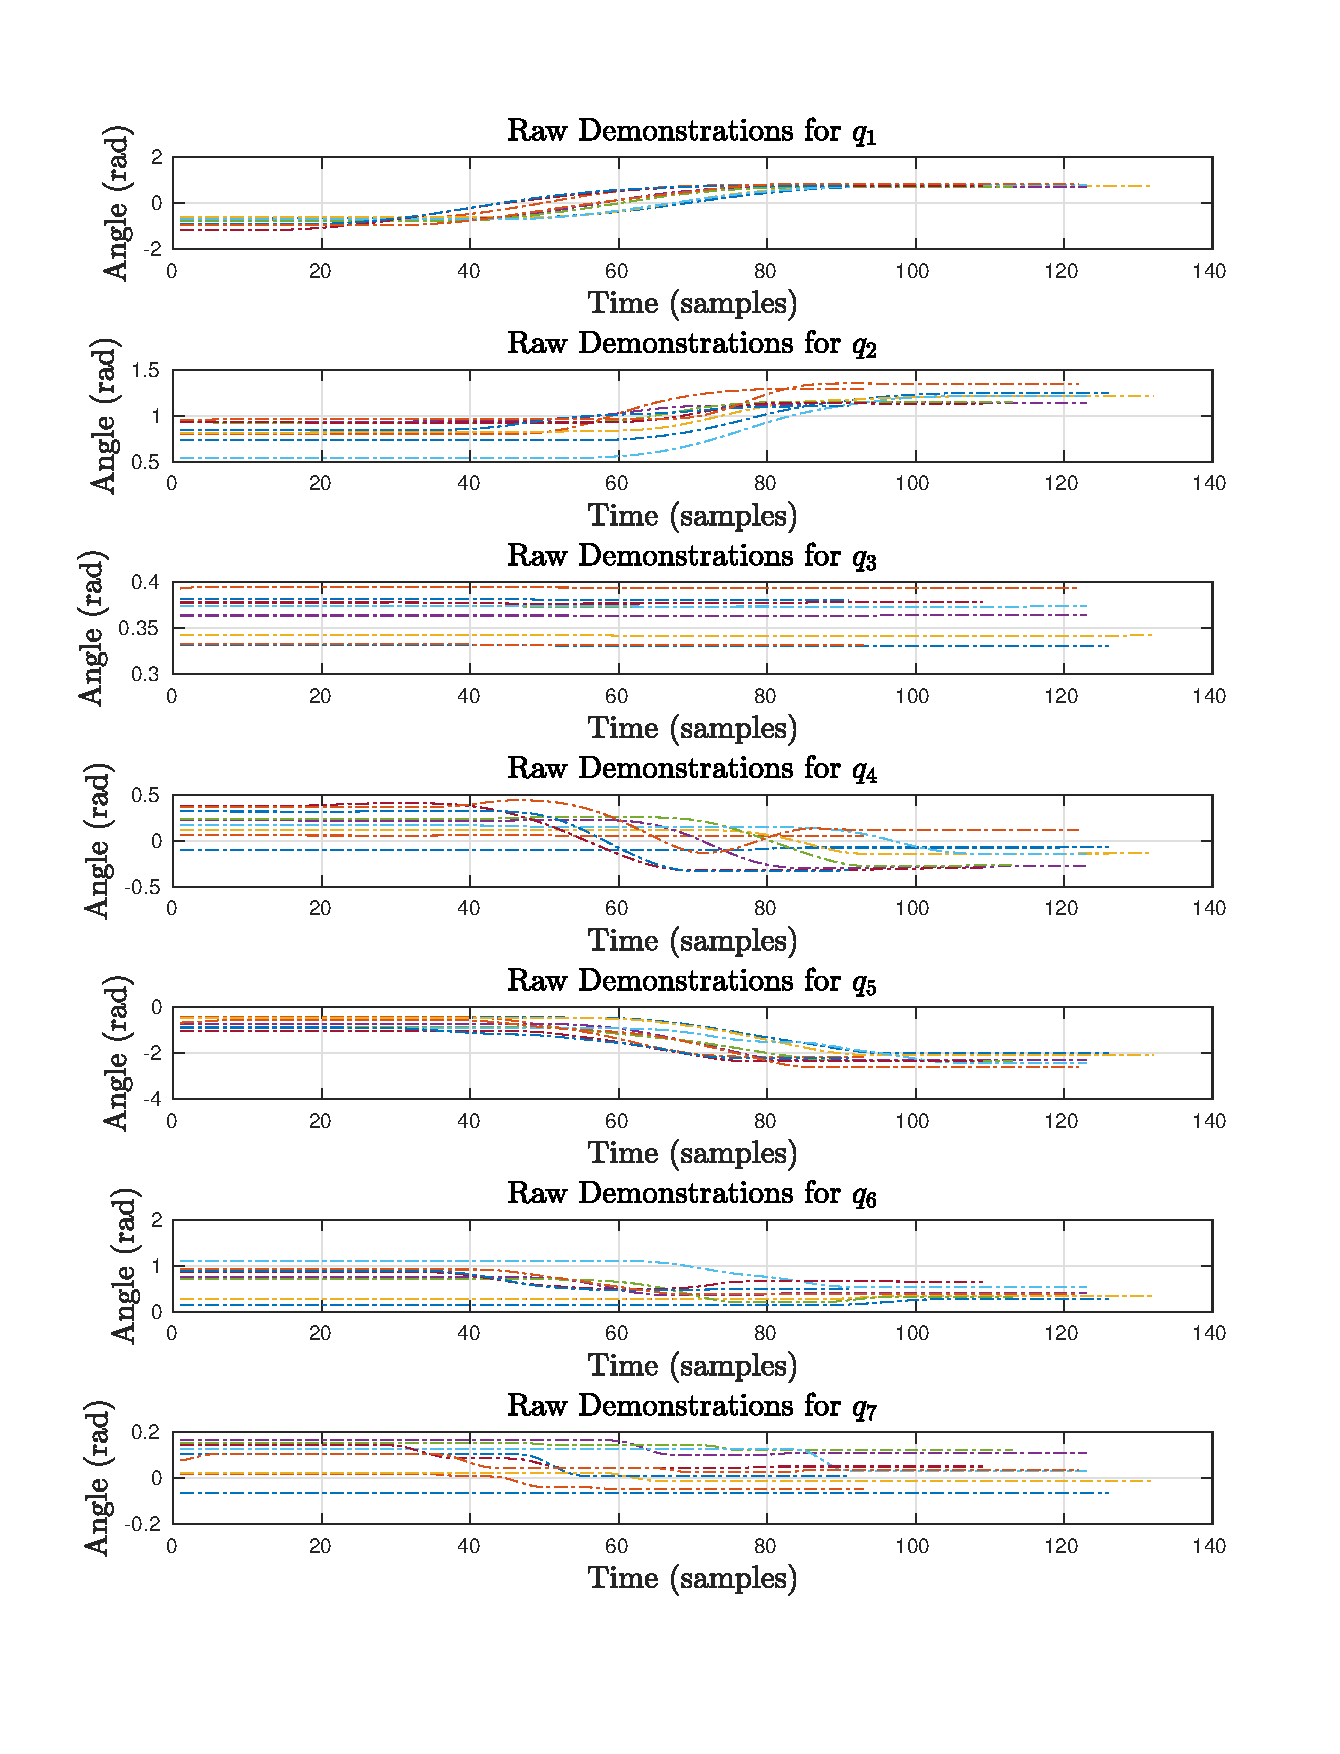
\includegraphics[trim={1.2cm 2cm 1.7cm 2cm},clip,width=\linewidth]{../../src/JTDS_mat_lib/figures/raw_demos_pour.pdf}
  \end{minipage}
   \begin{minipage}{0.47\textwidth}
      	\centering
      	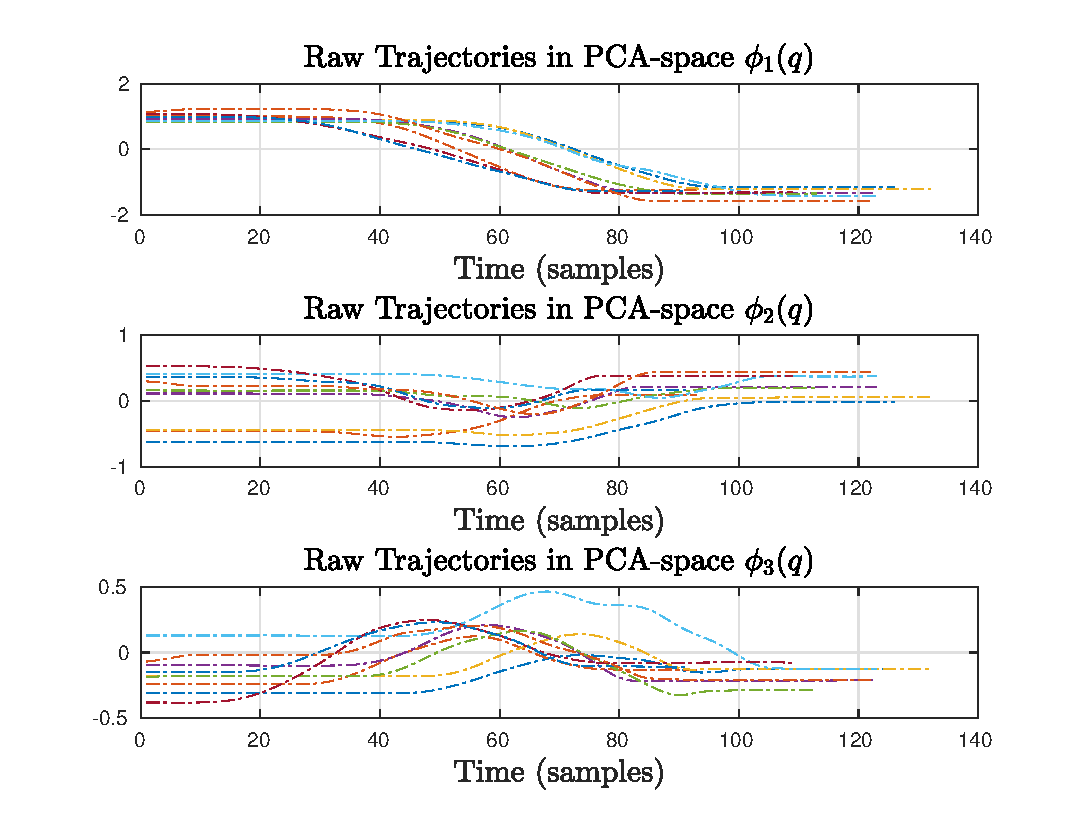
\includegraphics[trim={1.2cm 0.5cm 0.5cm 0.35cm},clip,width=\linewidth]{../../src/JTDS_mat_lib/figures/raw_demos_pca_pour.pdf}
      	\vspace{-5pt}
      	
		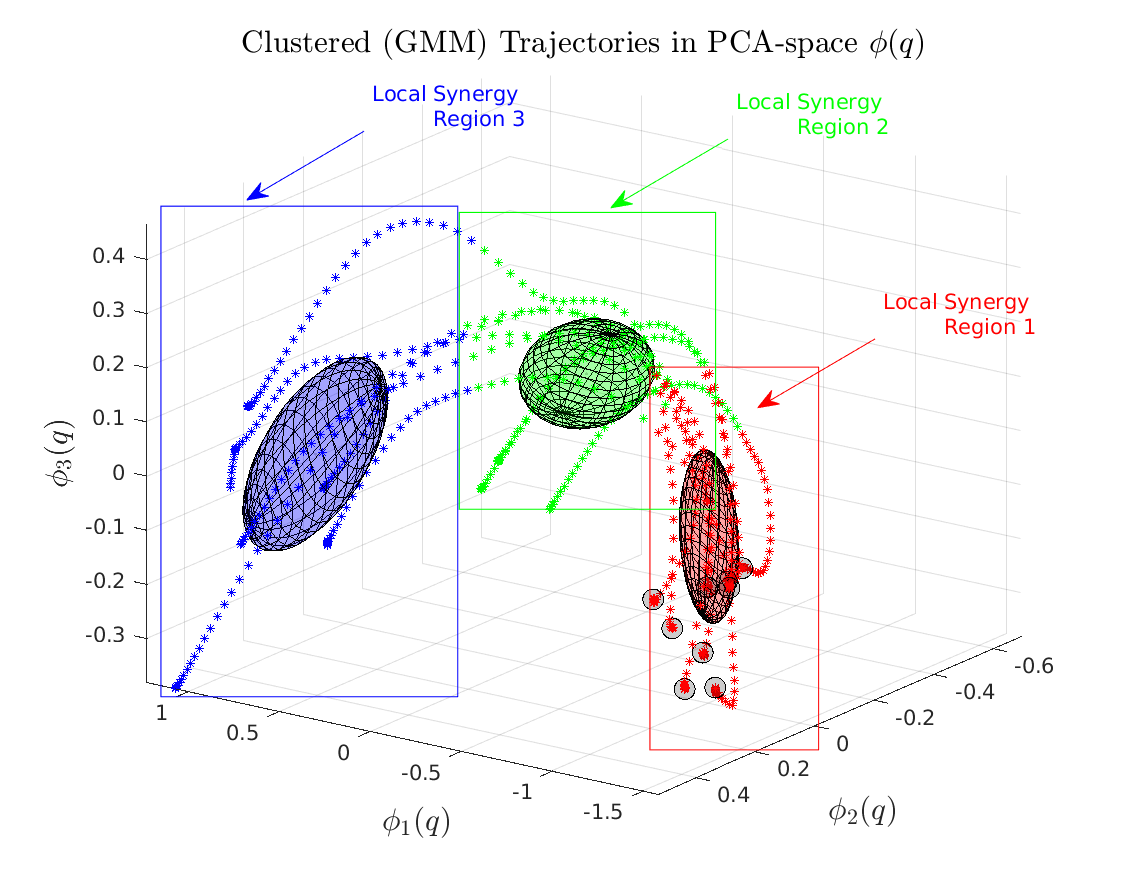
\includegraphics[trim={0.8cm 0.5cm 0cm 0.35cm},clip,width=\linewidth]{../../src/JTDS_mat_lib/figures/local_synergy_regions_pour_annotated.pdf}
   \end{minipage}
   \caption{Raw demonstrations of the pouring task in original space, PCA space and the extracted local synergy regions. \label{fig:raw_demos}}
\end{figure*}

\underline{As mentioned in the reviewers 3rd comment}, since we have an accurate representation of our joint posture trajectories and the local synergy regions in this lower-dimensional space, why not learn the $A_k$ matrices in this space; i.e. $\mathcal{A}(q)\in \mathbb{R}^{p\times p}$ rather than $\mathcal{A}(q)\in \mathbb{R}^{m\times m}$ ? This seems like the obvious method, if we were considering our synergistic approach the classical way, i.e. using the lower-dimensional space as the new control variables. However, if we were to do that, this would mean that \eqref{eq:jtds} would become:
\begin{equation}
\underbrace{\dot{q}}_{\mathbb{R}^{m\times 1}} = -\underbrace{M_p^{-1}}_{\mathbb{R}^{m\times p}}\underbrace{\mathcal{A}(q)}_{\mathbb{R}^{p\times p}}\underbrace{M_p}_{\mathbb{R}^{p\times m}}\underbrace{J^{T}(q)}_{\mathbb{R}^{m\times d}}\underbrace{(H(q)-x^*)}_{\mathbb{R}^{d\times 1}}
\label{eq:jtds_low}
\end{equation}
This is not entirely incorrect, however, with such a control law we can no longer guarantee stability and convergence to the attractor $x^{*}$. By considering the Lyapunov function used in Appendix I to prove stability of \eqref{eq:jtds_low} i.e. $V(q) = \frac{1}{2}(H(q) - x^*)^T(H(q) - x^*)$, the derivative of $ V $ wrt. would be:
\begin{equation}
\begin{aligned}
\frac{dV(q)}{dt} &= (H(q) - x^*)^TJ(q)\dot{q}\\
&= -(H(q) - x^*)^TJ(q)M_p^{-1}\mathcal{A}(q)M_pJ^T(q)(H(q) - x^*)\\
&= -(H(q) - x^*)^TJ(q)\textcolor{red}{\underbrace{M_p^{-1}\big(\sum_{k=1}^{K}\underbrace{\theta_k(q)}_{> 0}\underbrace{A_k}_{\succ 0}\big)M_p}_{\text{This should be}~~ \succ 0}}J^T(q)(H(q) - x^*)\leq 0
\end{aligned}
\end{equation}
In order for \eqref{eq:jtds_low} to be asymptotically stable wrt. the attractor $x^*$ the term $M_p^{-1}\big(\sum_{k=1}^{K}\theta_k(q)A_k\big)M_p \in \mathbb{R}^{m\times m}$ should undoubtedly be $\succ 0$. Even if $\theta_k(q) > 0$ and $A_k \succ 0$ for all $k$, the only way for this condition to hold is if $M_p$ where a full symmetric positive definite matrix. However, this is not the case because $M_p\in \mathbb{R}^{p\times m}$  is a projection matrix, i.e. $p<m$. The term $M_p^{-1}\big(\sum_{k=1}^{K}\theta_k(q)A_k\big)M_p$ will no longer be full-rank, it will preserve the $p$ positive eigenvalues from the $A_k$ matrices, but the remaining eigenvalues will be 0, thus generating a semi-positive definite matrix, which invalidates our stability proof. Note that, as described in the Appendix, $J(q)$ is not proven to be full rank in all regions of the workspace, when this happens, this means that the end-effector pose is not manipulable. Hence, we can only prove asymptotic stability when the end-effector pose is manipulable. This is a physical artifact from the joint-space constraints of the robot arm which we cannot avoid. Yet, since the demonstrations are acquired via kinesthetic teaching we can assume that they are manipulable. \underline{As asked by the reviewer, what does it physically mean to have all positive eigenvalues?}  When \\ $M_p^{-1}\big(\sum_{k=1}^{K}\theta_k(q)A_k\big)M_p$  or ($\mathcal{A}(q)$) has some eigenvalues $=0$ the physical meaning behind it is that we are forfeiting the control of these directions of motion in joint-space. Namely, the desired velocity directions in joint-space will be constrained in the corresponding DOF of the arm, this will prohibit us from converging to the attractor and will be no longer capable of accurately following the joint-space demonstrations.  If instead we learn the synergy matrices in joint-space following \eqref{eq:jtds} and modulate them with the activation function in PCA-space, we avoid all of this problems and can ensure full controllability of the motion in joint-space. 

\noindent \textbf{Remark 1:} This analysis is only considering PCA as the DR approach. If we would consider K-PCA, deriving such a control law is more involved as the inverse mapping $\phi(q)^{-1}$ is not straightforward if at all possible, thus limiting the approach to linear DR techniques. By considering $\phi(q)$ solely in the activation function $\theta(\cdot)$ we do not have this problem and can use any DR technique, as long as we're able to compute out-of-sample projections.

\noindent \textbf{Remark 2:} If we were to bypass the DR step our state-dependent system matrix would become $\mathcal{A}(q)= \sum\limits_{k=1}^{K}\theta(q)A_k$, which (via our definition) is also a combination of ``local behavior synergy matrices" with the activation function living in joint-space rather than the PCA space; better-known as the \textit{joint postural synergy space}. The fact that we use PCA/K-PCA to represent the activation function $\theta(\cdot)$ is to alleviate the complexity of extracting the local synergy regions in joint-space directly. It is, indeed, also motivated by the fact that we know that multi-DOF joint postures can be accurately represented in a lower-dimensional space composed of the principal components of the postural trajectories; i.e. the well-known \textit{joint postural synergies}. As shown in TABLE I of the manuscript and discussed in Section V, by using a lower-dimensional manifold to represent the joint trajectories, we are getting rid of outliers, noise and redundancies that might arise from the raw joint demonstrations. This is explicitly highlighted in Section V:\\
\textcolor{blue}{\small \textit{"As can be seen, for all datasets there is a significant increase in performance on the testing sets when using either dimensionality reduction (DR) approaches. This suggests that using DR to encode our activation functions $\theta_k$ in a lower-dimensional space $\phi(q)$ yields better generalization capabilities than encoding the behaviors in using the original $q$. This is most notable for the three pouring motions, where the joint-velocity RMSE testing error for a JT-DS model learned without DR is an order of magnitude higher than with DR. Such an error indicates that the demonstrated joint-behavior was over-fitted on the training set, which is also exhibited in the higher number of $K$ needed to represent the motion without DR. For all datasets, the DR methods provided $\delta < d/2$, either comparable or less number of local behaviors synergies $K$ and better RMSE errors on testing sets as opposed to no DR. By finding a lower-dimensional manifold to represent the joint trajectories, we are getting rid of outliers, noise and redundancies that might arise from the raw joint demonstrations. Hence, through DR we are capable of robustly extracting the local behavior synergies from raw demonstrations."}} \\
Hence, through DR we are capable of robustly extracting the local behavior synergies from raw demonstrations and learn a \textit{time-invariant} controller that ensures reaching the task-space target while approximately following the demonstrated motion, as shown in Fig. \ref{fig:jtds_velocities}, where we plot the joint positions/velocities of 1 demonstrations of the pouring task and the joint-positions/velocities from the JT-DS controller. In these plots, we are taking the velocity generated directly by JT-DS. The joint-positions are then computed by numerical integration of these velocities. Note that our controller does not generate this entire trajectory in one-shot, it is generating the next desired velocity given the current joint posture, e.g. $\dot{q}_{t+1} = \mathcal{A}(q_{t})J^T(q_{t})(H(q_{t})-x^*)$ with $q_t$ being the current joint configuration. Moreover, our controller is state-dependent only; i.e. it has no dependence on time or the duration of the desired trajectories. Hence, it can generate motions similar to the demonstrated ones at different frequencies and time durations. 

\noindent \textcolor{red}{TODO: Add clarifications in text such that no other reader gets confused with the new concept of behavior synergies that we propose as opposed to the classical joint posture synergies.}



\begin{figure*}[!th] 
  \begin{minipage}{0.5\textwidth}
     	\centering 
     	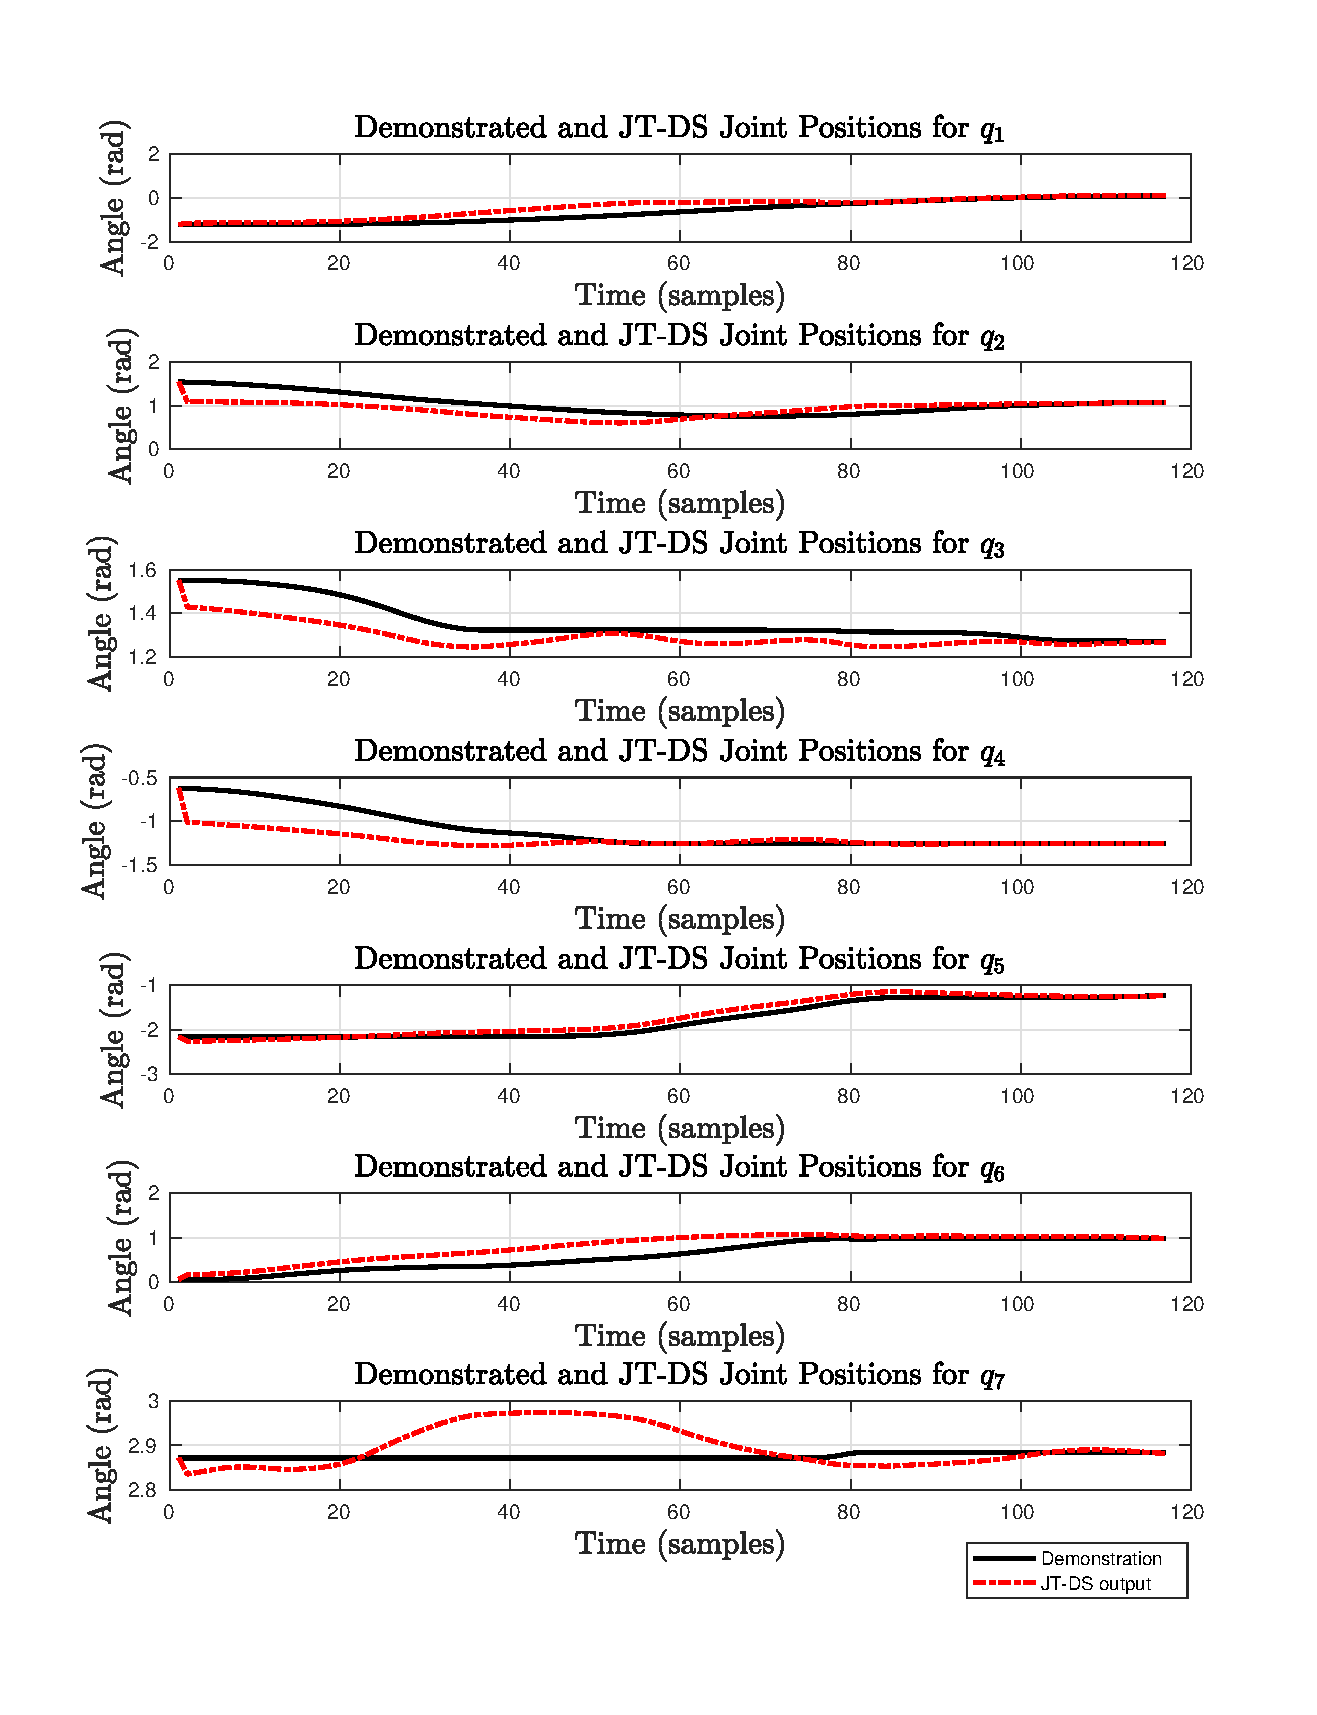
\includegraphics[trim={1.2cm 1.5cm 1.7cm 1.5cm},clip,width=\linewidth]{../../src/JTDS_mat_lib/figures/jtd_pos_pour1.pdf}
  \end{minipage}
    \begin{minipage}{0.5\textwidth}
       	\centering 
       	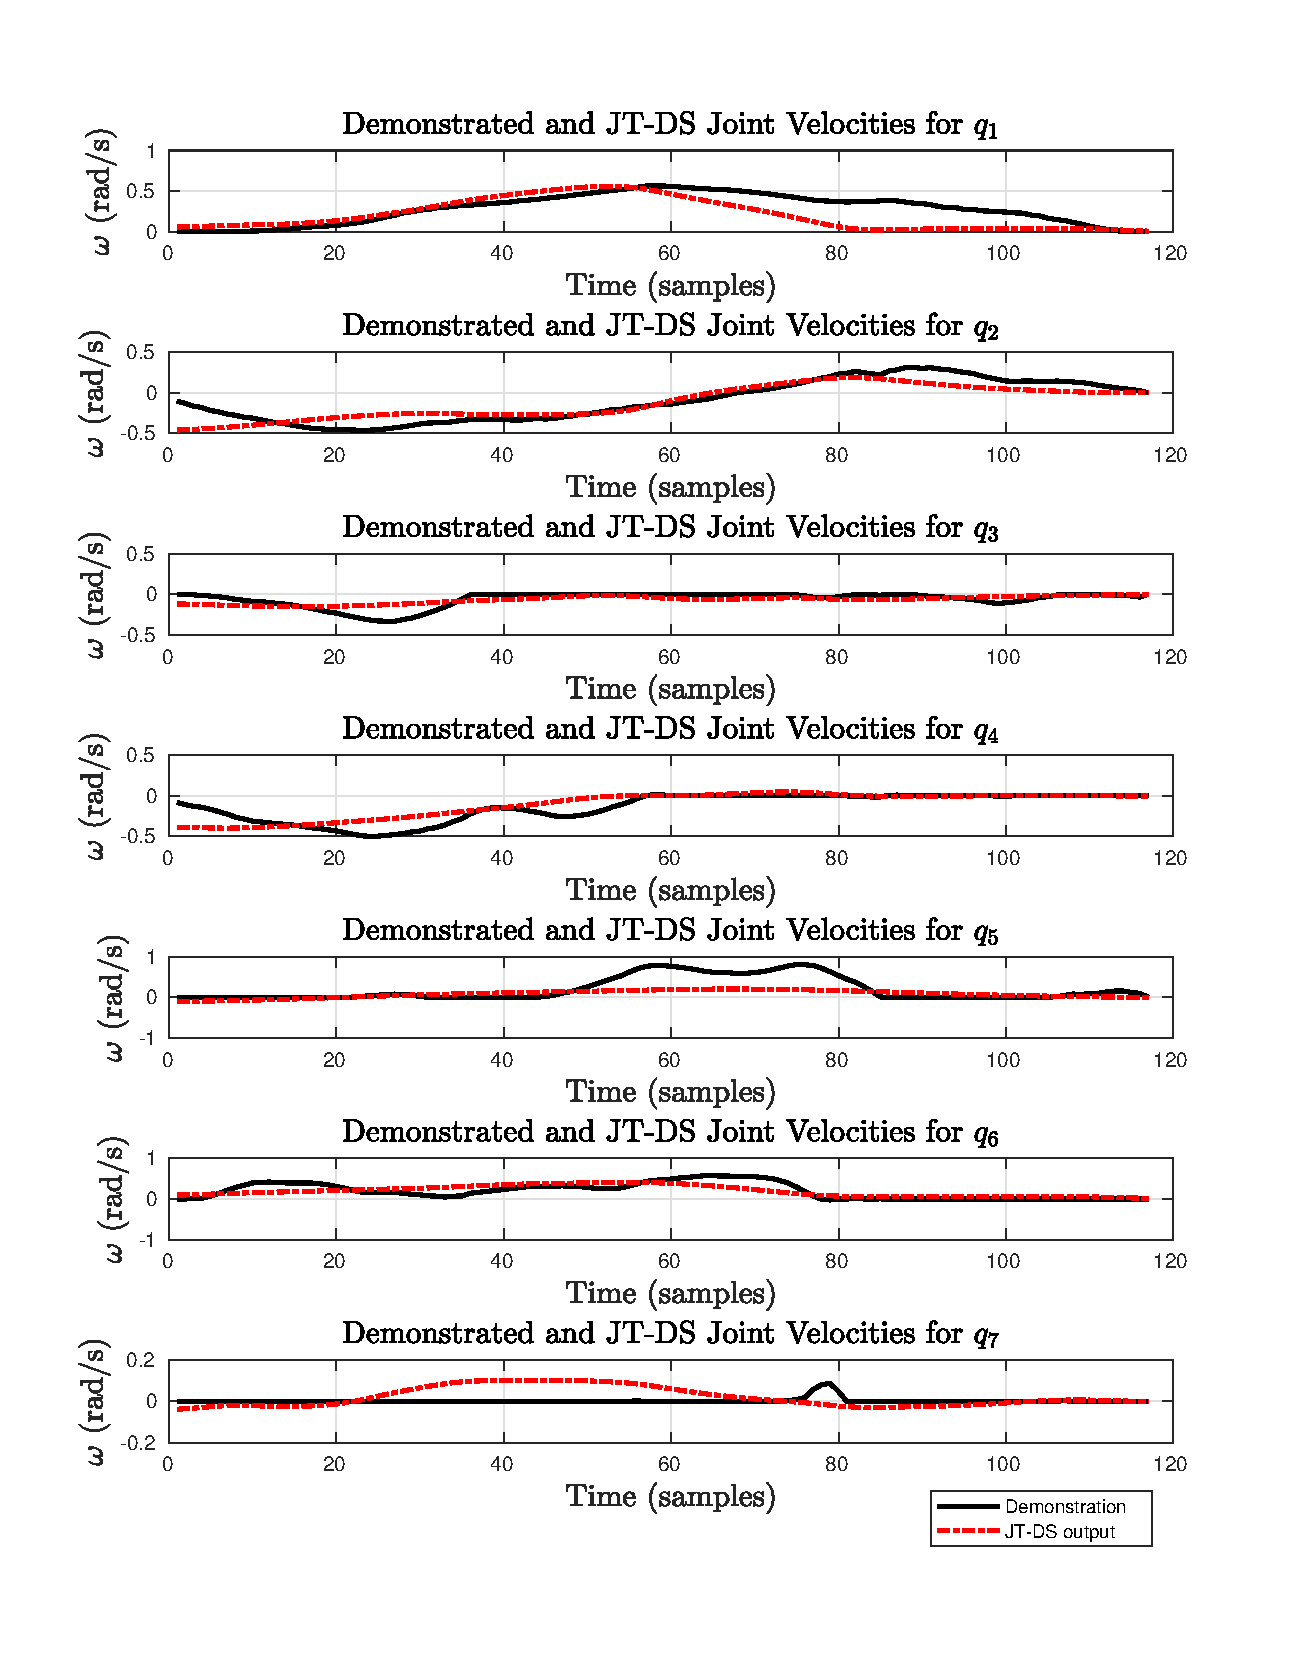
\includegraphics[trim={1.2cm 1.5cm 1.7cm 1.5cm},clip,width=\linewidth]{../../src/JTDS_mat_lib/figures/jtd_vel_pour1.pdf}
    \end{minipage}
   \caption{Training and executed joint-position/velocities with JT-DS for 1 pouring demonstrations. \label{fig:jtds_velocities}}
\end{figure*}
\newpage
\noindent \underline{On the applicability of F-PCA to our learning scheme:}  If we were to ignore our proposed control scheme and try to reconstruct the trajectories from the joint postural synergy components; i.e. using PCA, we would get the trajectories shown in Fig. \ref{fig:pca_velocities}. In these plots, we are taking one of the collected demonstrations projected in the PCA-space, i.e. $\phi(\{q_1,q_2,\dots,q_T\})$ and reconstructing it to generate the desired joint posture trajectories. To compute the velocities we apply numerical differentiation on the reconstructed joint positions. As can be seen, we are capable of generating similar trajectories, both in position and velocity. In this simple example we are saving the entire demonstration in PCA-space, however, if we were to use this for controlling the real robot we need to learn a model or a controller in this low-dimensional space and then map it back to joint-space. As discussed earlier, this is not feasible with our proposed control-law \eqref{eq:jtds}, due to the stability and convergence objectives we defined. 

\begin{figure*}[!th] 
  \begin{minipage}{0.485\textwidth}
     	\centering 
     	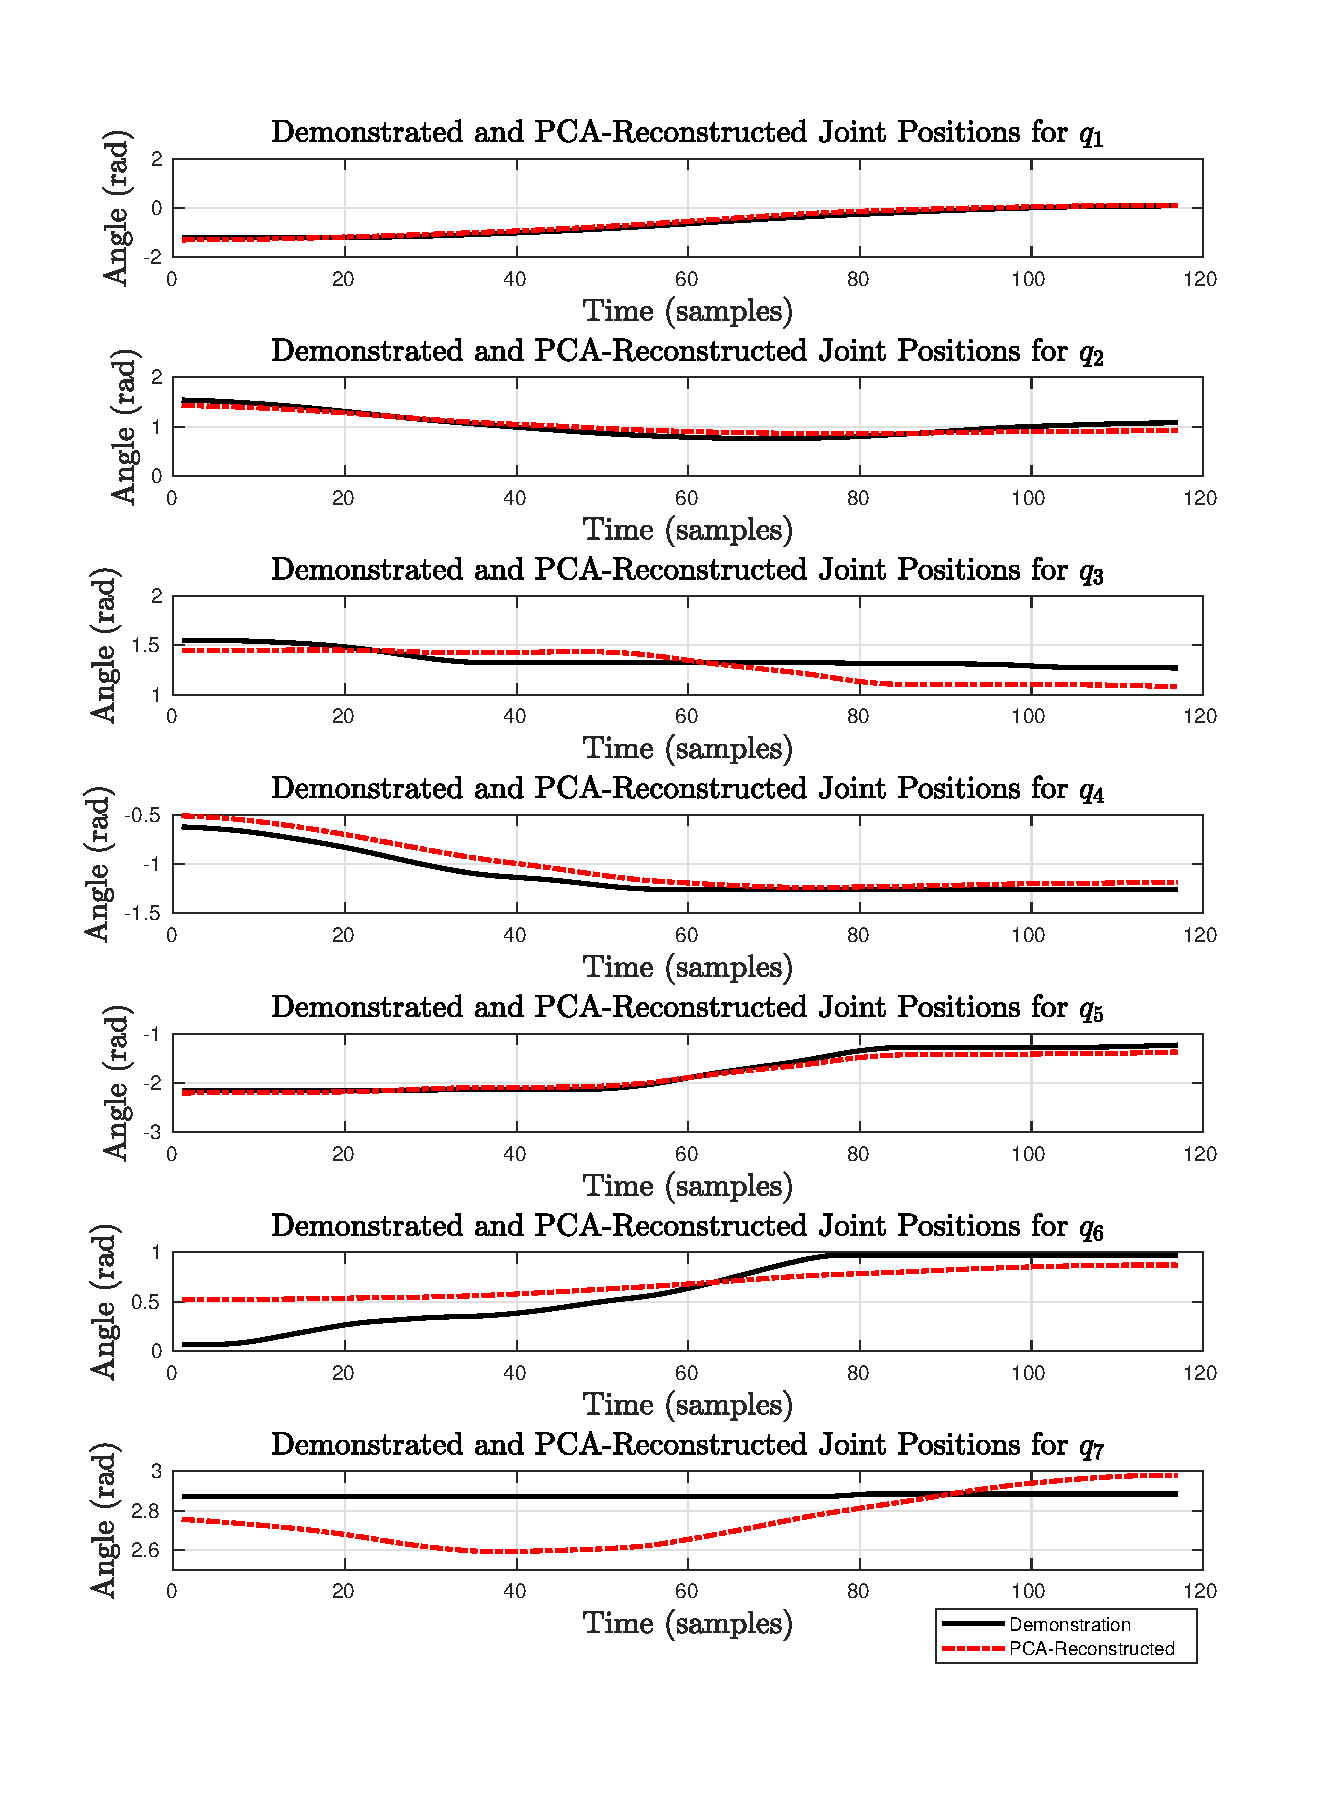
\includegraphics[trim={1.2cm 1.5cm 1.7cm 1.5cm},clip,width=\linewidth]{../../src/JTDS_mat_lib/figures/pca_pos_pour1.pdf}
  \end{minipage}
    \begin{minipage}{0.5\textwidth}
       	\centering 
       	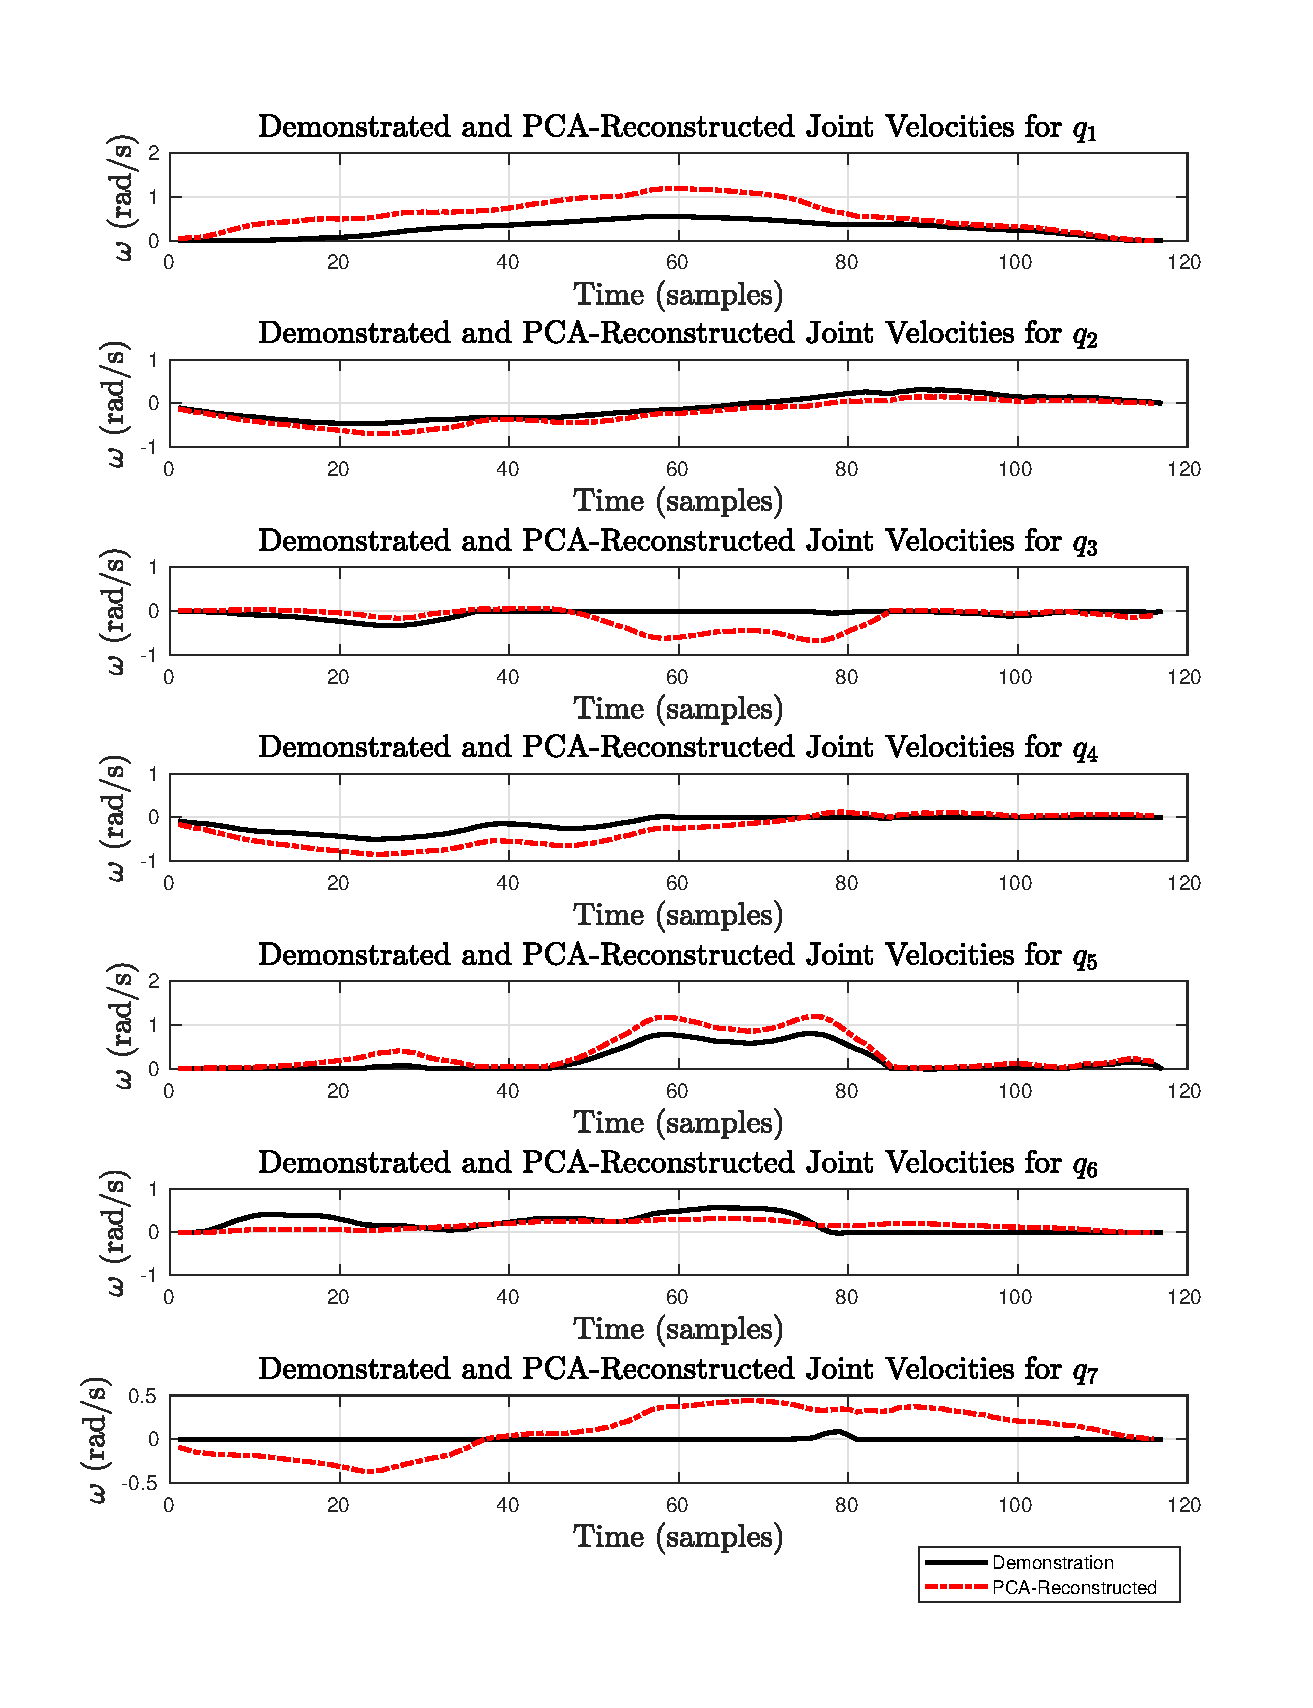
\includegraphics[trim={1.2cm 1.6cm 1.7cm 1.6cm},clip,width=\linewidth]{../../src/JTDS_mat_lib/figures/pca_vel_pour1.pdf}
    \end{minipage}
   \caption{Training and reconstructed joint-position/velocities with PCA for 1 pouring demonstrations. \label{fig:pca_velocities}}
\end{figure*}

Ignoring this limitation, one of the main draw-backs of this type of synergistic control is that the extracted representation in PCA space does not take into account the dynamic features of the motions and further assumes that the demonstrations have no time correlation. As mentioned by the reviewer and applied in \cite{Dai:IROS:2013} for modeling grasping motions and in \cite{Averta:FRAI:2017} for upper-limb motions, functional-PCA is a nice alternative to include these dynamic features and further reconstruct entire trajectories with a linear combination of a few \textit{time-dependent} functions. In this approach each demonstrated trajectory (of a single DOF) is considered as a function composed of a linear combination of $N$ basis elements (which can ve exponentials, splines, Fourier) $f_i = \sum\limits_{n=1}^{N}\theta_nb_N$. Thus, each $i$-th function (i.e. $i$-th demonstration) can be described by the vector a coefficients $\Theta = \{\theta_1,\dots,\theta_N\}$. PCA is then performed on $\Theta = \{\theta_1,\dots,\theta_N\}$ and the extracted PC are transformed to \textit{functional PCs} via the $N$ basis functions. Then $M<N$ \textit{functional PCs} are used to reconstruct the $i$-th function (i.e. $i$-th demonstration ) as $\hat{f}_i = \bar{f_i} + \sum\limits_{i=1}^{M}c_i\xi_i$, where $\bar{f}_i$ is the mean function, $c_i$ are the coefficients and $\xi_i$ are the \textit{functional PCs}. As shown in \cite{Averta:FRAI:2017} with only 1 \textit{functional PCs} 60/70\% of the demonstrations can be accurately reconstructed. This approach would be interesting if our goal were to reconstruct entire time-dependent trajectories as they do in  \cite{Dai:IROS:2013} and \cite{Averta:FRAI:2017}. This is, however, NOT our goal and applying this method to our control scheme seems not suitable and is rather an alternative approach for the following reasons: First of all, in this work we propose a DS-based controller, meaning that, we do not generate the full reference trajectory of the robot \textit{a prior} and then try to track it, we instead compute the next desired velocity on-the-fly which happens to result in the desired motion because it is encoded in $\mathcal{A}(q)$. Second, if we were to apply this method as the reviewer suggests, the only way to do it is to re-write a controller that uses 7 reconstructed functions $\hat{f}_i$ (i.e. one per joint) to track a time-indexed reference joint trajectory. This is a valid approach, however, in this work we propose a state-dependent; i.e. time-invariant approach. Finally, our goal not to accurately reproduce the demonstrations but rather to reach the target $x^*$ with a similar joint motion as the one that was demonstrated.

\item \textcolor{blue}{\textit{``For the test, why not comparing also with the JT control method? In
other terms, is it possible to use a SEDS + JT, especially for the
third case "Transiting through singular configurations"?"}}\\
\texttt{Response:} \small This could be done, but it is mathematically incorrect. The original JT control method is a DS that converges to a unique equilibrium point, i.e. the task-space target $x^*\in \mathbb{R}^{N\times 1}$, with a gain matrix $K \in \mathbb{R}^{M\times M}$ as:\begin{equation}
\dot{q} = K J(q)^T(H(q)- x^*) 
\label{eq:JT}
\end{equation}
SEDS on the other hand, is a DS-based motion generator that converges also to a unique equilibrium point, as:
\begin{equation}
\hfill \begin{aligned}
&  \dot{x}  = \mathbf{f}(x)
\rightarrow  &
\begin{cases}
\lim_{t \rightarrow \infty}\|x - x^*\|=0
\end{cases}
\end{aligned}  \hfill
\label{eq:simple-ds}
\end{equation}
where $\mathbf{f}(\cdot): \mathbb{R}^M \rightarrow \mathbb{R}^M$ is a continuous differentiable vector-valued function representing a non-linear DS that converges to a single stable equilibrium point $x^*$. SEDS is used in the following way: Given the current state of the robot $x$ the next desired velocity $\dot{x}_d$ is computed with \eqref{eq:simple-ds} this is then fed to a velocity-based IK solver as shown in Fig. \ref{}:\\
\textcolor{red}{TO SINA: Include typical SEDS-like control-loop here}\\
If we were to use SEDS with the JT-control method, we would have to integrate the desired velocity to generate a desired position $x_d$ at each time-step and define it as the target in \eqref{eq:JT}, which would yield the following controller:
\begin{equation}
\dot{q} = K J(q)^T(H(q)- x_d) 
\end{equation} Note that, the JT control method assumes that the target is static, hence, in order for this controller to actually converge, the output of \eqref{eq:simple-ds} must seem constant for a period of time. This is contradicting as \eqref{eq:simple-ds} is always trying to converge to $x^*$. Thus, merging these two approaches is theoretically ill-fitting. To better highlight this, we show an illustration of the supposed SEDS+JT control loop in Fig. \ref{}:\\
\textcolor{red}{TO SINA: Include SEDS+JT control-loop here}\\
\textcolor{red}{\small Describe this control-loop and state more reasons (if any) why it's wrong...}

\item \textcolor{blue}{\textit{``Minors:
- SEDS + IK: what does SEDS mean?"}}\\
\texttt{Response:} As stated in the previous comment, SEDS, short for Stable Estimator of Dynamical Systems is an approach proposed in \cite{khansari2011learning} that learns a stable estimate of a DS with the form of \eqref{eq:simple-ds} from demonstrations. The first paragraph of Section V.B was written to describe its meaning and how we use it:\\
\textcolor{blue}{\small \textit{``We now seek to elucidate the distinctive properties of our JT-DS model by comparing its performance to a DS-based Cartesian motion generator + IK solver approach for behaviors \textit{(5-7)}. For the Cartesian motion generator we use the SEDS (Stable Estimator of Dynamical Systems) approach [8] which learns an asymptotically stable DS in Cartesian space from demonstrations. We then generate joint trajectories through a damped least square IK solver. From herein we refer to this approach as SEDS+IK."}}\\
\end{enumerate}
% % % % % % % % % % % % % % % % % % % % % % % % % % % % % % % % % % % % % % % % % % % % % % % % % % % % % % % % % % % % % % % % % % % % % % % % % % % % % % % % % % % % % % % % % % % % % % 

\underline{Comments from Reviewer \#3 (Reviewer: 7 (Review30521)):}
\begin{enumerate}
\item \textcolor{blue}{\textit{``a considerable part of the introduction is spent in comparing joint space trajectory generation to task
space trajectory generation. Since these are elementary concepts in robotics, the authors might consider
reducing this part"}} \texttt{Response:} Several sentences in the introduction have been removed/reduced.\\

\item \textcolor{blue}{\textit{``one of the main claims of the paper is the stability proof, which in fact is cited in the first line of the
abstract. However the stability analysis is a quite simple extension of the stability of the transpose
Jacobian scheme, where the constant gain on the task space error is replaced by the matrix A(q). As
such the emphasis on this result might be to some extent reduced. By the way, the proof works only
if the Jacobian is full rank, which is not properly discussed in Appendix I"}}\\
\texttt{Response:}  Removed a couple mentions of the stability result, and added the dependence on the rank of the Jacobian to both the appendix and the main body of the text.\\

\item \textcolor{blue}{\textit{``the meaning of variables $q_d$ in (2) is not very clear to me, a well as whether it takes the same meaning
as $q_{t;n}$ in (8)"}}\\
\texttt{Response:} $q_d$ are the velocities from the demonstrations, which we are aiming to recreate. Equation (8) has been updated to remove the typo (they are in fact the same).\\

\item \textcolor{blue}{\textit{``Section III uses the concept of synergy without actually defining it. An introduction to this concept is given later, in Section IV"}}\\
\texttt{Response:} Added the following to Section 3:\\
\textcolor{blue}{\small \textit{``Each ``synergy" is a joint-space transformation that biases the resulting motion to use particular joints; for more, see Sec. IV."}}\\

\item \textcolor{blue}{\textit{``the expression "flow of motion" in Proposition 1 is not very clear to me"}}\\
\texttt{Response:}  Changed to "motion".\\

\item \textcolor{red}{\textit{`some details about the optimization problem in (8) might be given
(nature of the problem, complexity, feasibility)."}}\\
\texttt{Response:} The following has been added near Eq. (8):\\
\textcolor{blue}{\small \textit{``The resulting optimization minimizes the mean squared joint velocity error from \eqref{eq:optim_error}, resulting in a convex semidefinite optimization with a quadratic objective..." ``This optimization is always feasible (the only constraint is that the $A_k$s be independently PSD), and the number of terms in the objective is $O\left(k^2d^3\left( \sum_{n=1}^N T_n\right)\right)$."}}\\
To elaborate about the prior calculation: the number of terms in the sum is proportional to the number of recorded points, times the number of matrices (k) required to generate the predicted velocity from (7) squared, times the number of terms in a matrix multiplication of two $d x d$ matrices ($d^3$).\\

\end{enumerate}



\bibliographystyle{plain}
\bibliography{Refs.bib}

\end{document}

